% $Id: Presentation-FCSM2013-appendix.tex 405 2013-11-05 00:53:34Z lv39 $ 
% $URL: https://forge.cornell.edu/svn/repos/ncrn-cornell/branches/papers/FCSM2013/DDI-PROV/Presentation/Presentation-FCSM2013-appendix.tex $ 

\section{Extra slides}
\frame{\tableofcontents[currentsection]}

\subsection{Census Bureau}
\begin{frame}[label=Census]
\frametitle{Dataset usage in Census RDC}
\begin{block}{1,505 project-dataset pairs}
\centering
%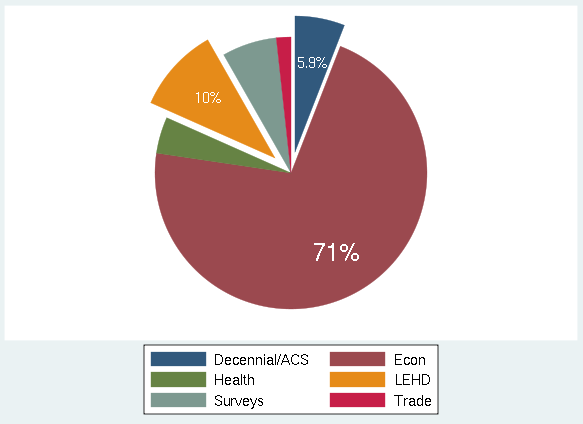
\includegraphics[width=0.8\textwidth]{../pie-chart-rdc-data}
\end{block}
\tiny Many projects use multiple datasets.
\end{frame}

\begin{frame}
\frametitle{Economic (business) datasets}
\begin{itemize}
\item 71\% of datasets are business (economic) datasets
\item Primarily establishment-based records from the
Economic Censuses and Surveys, the Business Register, and the Longitudinal Business Database (LBD)
\item They form the core of the modern
industrial organization studies \cite%
{DunneRobertsSamuelson1989,OlleyPakes1996} as well as modern gross job
creation and destruction in macroeconomics \cite%
{DavisHaltiwangerSchuh,HaltiwangerJarminMiranda2010}.
\item But there are no public-use micro-data for these establishment-based products
\item Exception: recently-released Synthetic LBD \cite%
{AbowdVilhuber2010,KinneyEtAl2011}
\item Currently no active curation (of derived datasets) [a], no way to reference [b], convoluted way to learn about the data structure [c$^*$]
\end{itemize}
\end{frame}

\begin{frame}
\frametitle{LEHD data}
\begin{block}{Linked employer-employee data}
\begin{itemize}
\item Longitudinal and cross-sectional detail
\item New confidentiality protection methodologies \cite{AbowdEtAl2012,Ashwin2008}
have unlocked large amounts of data for public-use: highly detailed local area tabulations
exist based on the {LEHD} data
\item But: no public-use micro-data exist for this
longitudinal job frame or any of its derivative files.
\item Confidential data are dynamic (quarterly changes)
\item Currently some active curation (archiving, 10-yr!) [a$^*$], no way to reference (publicly) [b$^*$], convoluted way to learn about the data structure [c$^*$]
\end{itemize}
\end{block}
\end{frame}
\subsection{IRS}
\begin{frame}[label=IRS]
\frametitle{Not unique to Census Bureau}
\begin{block}{Internal Revenue Service/ Social Security Administration}
\begin{itemize}
\item
New projects (Chetty et al, 2012; von Wachter and co-authors) have created and/or used linked longitudinal data at the IRS or the Social Security Administration.
\item Neither agency has long-run experience at the statistical data curation function [a], (meta)data dissemination [b,c].
\item Although both IRS and SSA have produced statistical tables for a long time.
\end{itemize}
\end{block}
\end{frame}
\subsection{BLS}
\begin{frame}[label=BLS]
\frametitle{Not unique to Census Bureau}
\begin{block}{Bureau of Labor Statistics}
\begin{itemize}
\item Long history of making time-series available
\item Limited access to microdata at the BLS 
\item Unknown curation [a]
\item Even for public-use data, no way to reference specific releases [b]
\item No well-established way to learn about microdata [c]
\end{itemize}
\end{block}
\end{frame}

\subsection{CDER}
\begin{frame}[label=CDER]
\frametitle{Canadian Centre for Data Development and Economic Research}
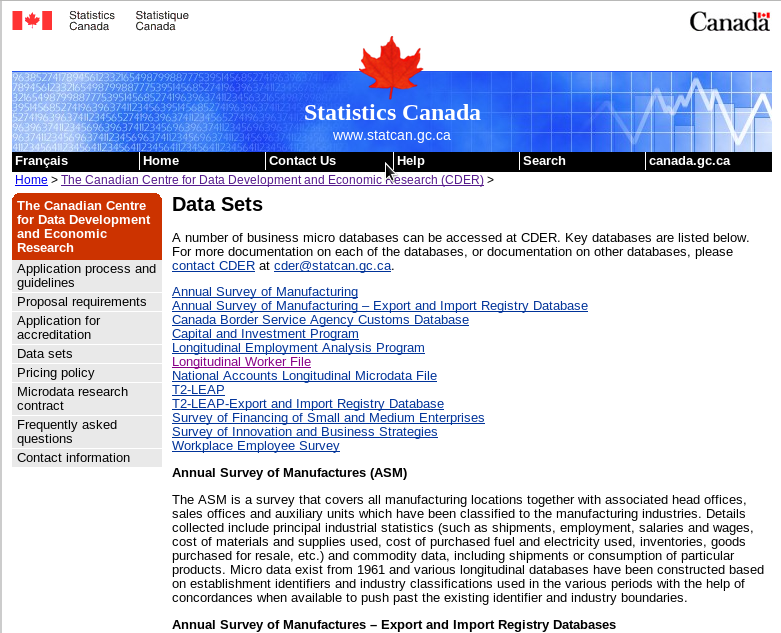
\includegraphics[width=\textwidth]{cder-20130804.png}
\end{frame}

\subsection{CRDC}
\begin{frame}[label=CRDC]
\frametitle{Canadian Research Data Centres}
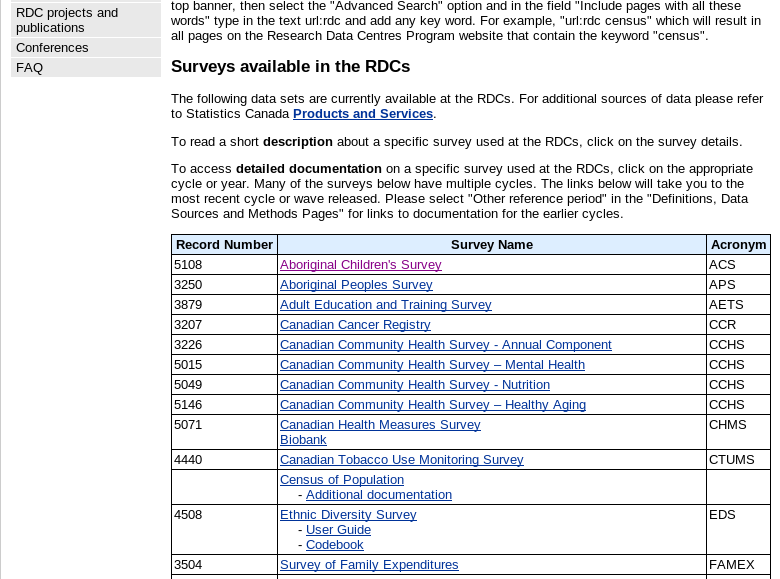
\includegraphics[width=\textwidth]{cdn-rdc-20130804.png}
\end{frame}

\begin{frame}
\frametitle{Canadian Research Data Centres}
\begin{block}{... but also not perfect}
Attempt to access data information on General Social Survey
\end{block}
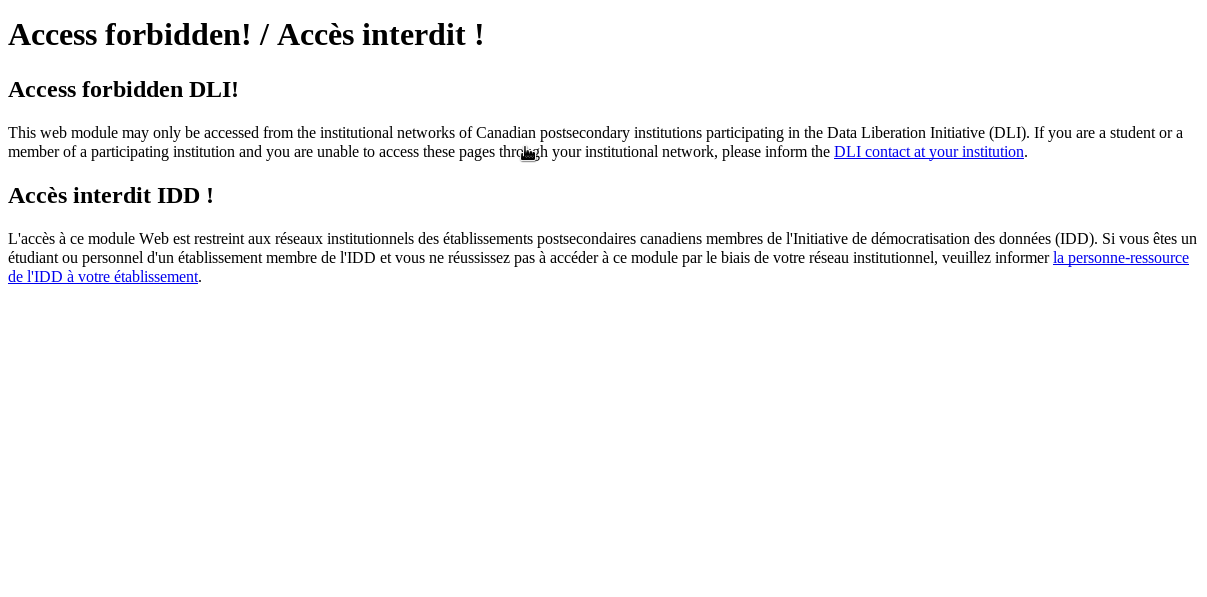
\includegraphics[width=\textwidth]{cdn-rdc-20130804-forbidden.png}
\end{frame}

\subsection{France}
\begin{frame}[label=France]
\frametitle{R\'eseau Quetelet}
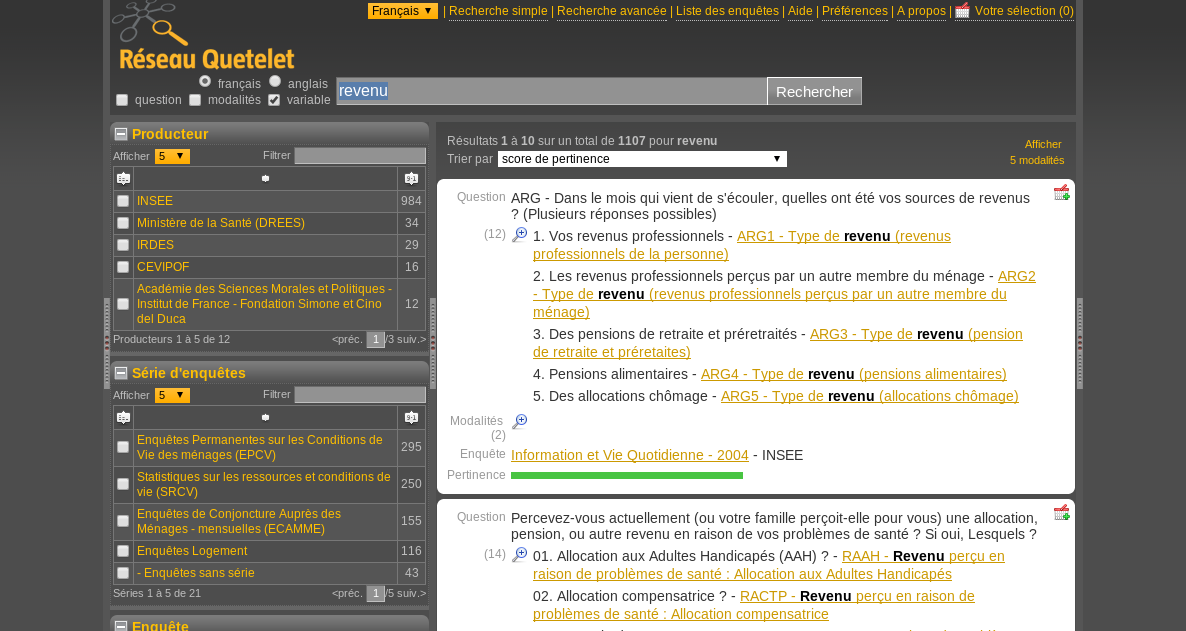
\includegraphics[width=\textwidth]{quetelet-20130804.png}
\end{frame}

\begin{frame}
\frametitle{}
\tiny
\bibliography{abbrev,paper}
\bibliographystyle{IEEEtranS}



\end{frame}
